\section{Planning an NDN}
\label{planning-ndn}
This section will discuss the method we used in order to plan an \gls{ndn} with scalability in mind. Scalability is defined as capacity to be changed in size or scale. In order to plan an \gls{ndn} with this goal in mind we will use a combination of McCabe's method (section \ref{overview-mccabe}) and \gls{tosca} (section \ref{overview-tosca}). McCabe will function as a method to guide design choices with scalability and performance requirements in mind. While \gls{tosca} will function as an implementation method that provides the means to control the whole life cycle of the network design and deployment. Furthermore, a proof of concept will be discussed that we implemented in a limited scope, in order to proof the method in practice. Furthermore, the method described in this section is deployed in a small scale proof of concept. However, the train of thought used for the \gls{ndn} design, planning and management can be applied to larger scale deployments, such as research clouds.

\subsection{Design requirements and analysis (McCabe)}
\label{planning-requirements}
In this section we will apply McCabe's approach in order to establish the design requirements and analyze the properties of \gls{ndn} and how it can be applied to solve the problem stated from section \ref{introduction-background}. A requirement is flexible scalability, this will be addressed by deploying and managing \gls{ndn} in an \gls{nfv}-style. Therefore, \gls{ndn} will be deployed as virtual functions and managed centrally via virtualization techniques as discussed in section \ref{overview-virtualization}. The first step is to make an overview of the requirements and known \gls{ndn} scalability and performance issues.

The following analysis is based on the design requirements and will provide a starting baseline for the high-level network design. As discussed in the related work (section \ref{introduction-related-work}), several key scalability and performance metrics were addressed. Several NDN-specific design choices need to be made. These include the consideration that \gls{ndn} is an overlay, on top of e.g. IP. Within this context it was concluded that TCP provided the most satisfying performance when compared to UDP. Furthermore, there are several \gls{ndn} strategies to choose from. The 'leave copy everywhere' cache decision strategy and the 'least recently used' cache replacement strategy were considered to be the overall best performing choices. However, for the forward strategies there was no decisive conclusion on which a selection could be based on. Therefore, we will use the default forwarding strategy; best-route. In terms of cache size, Koulouzis et al. recommends a cache size twice the size of the largest data object residing in the used repositories. The data catalogue or registry system provides metadata of digital objects, where the size and \gls{pid} type is available. This information may be used to sort the files in the catalogue by maximum size. The performance configurations mentioned can be configured in the \texttt{nfd.conf} file of the \gls{cxx} application. \gls{cxx} is one of the most mature software implementations of \gls{ndn} and therefore used in our design. Other performance optimization solutions which were mentioned in the related work require changes in the source-code. These source-code optimizations were not made public or are not yet integrated in existing software and therefore not used.

% add mulhouse and nimes hardware specs
The following recommendations are merely a baseline for research clouds and act as a starting point for performance optimizations, which is an iterative process. This process in practice should be based on the input values needed for McCabe's method discussed in section \ref{overview-mccabe}. However, these hardware configurations can be applied dynamically on cloud environments and adjusted to custom requirements. \gls{tosca} can be used to apply these changes from a central deployment and management description.

The following hardware requirements were determined based on the software documentation, the problem statement from section \ref{introduction-background} and related work from section \ref{introduction-related-work}. For VM memory requirements, 8-12GB and 2 CPUs or more are recommended. This was determined based on the recommended system requirements for Kubernetes \cite{kubernetes-system-requirements} and the fact that the use case may be I/O intensive. Therefore, I/O caching in memory benefits performance. In order to have sufficient disk space to cache \gls{ndn} data objects, install software, store logs and containers, a minimum of 100GB of storage is recommended.

\subsection{Architecture (McCabe)}
\label{planning-architecture}
With the design requirements established, we can develop a high-level network design. As mentioned in section \ref{overview-virtualization}, virtualization allows for flexible allocation of cloud resources via VMs while scalability of software applications can be realized by the use of containers in a \gls{nfv}-style. If more cloud resources are required, then this can be done by deploying more VMs. Furthermore, if needed, VMs can be deployed in specific geographically located cloud providers, expanding the data distribution availability. The virtual \gls{ndn} functions running inside these cloud providers, can then provide locally cached copies of data objects. And thus providing data distribution which lowers the chance of network congestion. In figure \ref{fig:high-level-network-design} we illustrate our high-level network design. In this illustration there are two conceptual cloud providers; 'mulhouse' and 'nimes'. These two nodes each are equipped with 12GB RAM and an Intel Xeon CPU E3-1240L v5 @ 2.10GHz with 1TB disks. In both of these conceptual cloud providers a VM will be deployed in order to allocate the resources needed.
% ADD DISK SIZES

\begin{figure}[H]
\centering
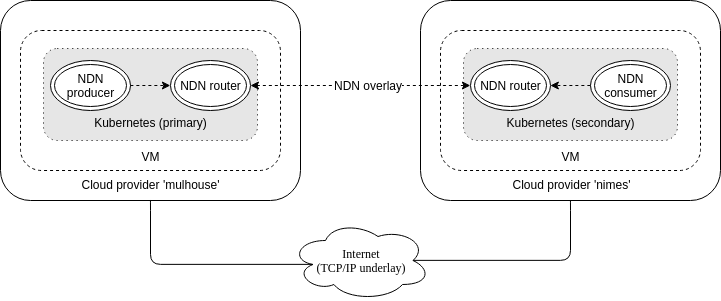
\includegraphics[width=\columnwidth]{Images/high-level-network-design.png}
\caption{High-level network design.}
\label{fig:high-level-network-design}
\end{figure}

Our high-level network design (figure \ref{fig:high-level-network-design}) contains three different virtual functions for \gls{ndn} nodes. The producer is assigned the function to make data available in the \gls{ndn}. The consumer is assigned to request data from the producer. However, in \gls{ndn}, any node that has named data, can reply to interest packets. So the producer and consumer functions can be interchangeable. The router's function is to forward interest packets between the two cloud providers. This forwarding is done in the \gls{ndn} overlay, which runs on top of the internet (underlay). \gls{ndn} is designed in such a way that any node can exchange named data, thus sharing between neighbours without a router is possible. However, a dedicated \gls{ndn} router offers a persistent presence in the \gls{ndn}, allowing forwarding control and maintain a stable dedicated cache.

% In summary; resources can be scaled in or out by deploying more VMs. In order to provide users a local \gls{ndn} cache, a regional cloud provider can be used to deploy a VM. By the use of Kubernetes, the \gls{ndn} application (node) can be scaled in and out as well. Where each \gls{ndn} node can be responsible for caching/forwarding a different subset of the naming hierarchy, in order to load-balance requests. 

These \gls{ndn} functions are deployed via a Kubernetes cluster (section \ref{overview-virtualization}), spread over the two conceptual cloud providers; ('mulhouse' and 'nimes'). These cloud providers are spread geographically in order to provide users with their regional \gls{ndn} cache. Kubernetes can be used to keep a central control over the \gls{ndn}, where pods (containers) can be created, removed and managed. These pods are spawned from images and custom tailored for their specific network function. This is done by the use of scripts running inside the containers, which configure the \gls{ndn} based on environment variables provided by Kubernetes, as described in section \ref{overview-virtualization}. Cache misses are expensive since they require an update of the cache, which puts load on the original publisher of the data, e.g. on SeaDataCloud or any other research cloud. Which is what we want to prevent. Therefore, pods preferably are configured with persistent data volumes (section \ref{overview-virtualization}), on which the cached data can be stored outside of the container. Kubernetes can also load-balance requests between a set of identical pods. However, if these pods do not share the same persistent cached data, cache misses may occur, which results in performance degradation.

\subsection{Deploying an NDN (McCabe and TOSCA)}
\label{planning-deploying}
Now that the network analysis, design and architecture are defined, a deployment strategy is needed. The high-level design (figure \ref{fig:high-level-network-design}) needs to become deployable with a scalable method. Scalable in this context means that a single deployment strategy can be used for different cloud providers. As described in section \ref{overview-tosca}, \gls{tosca} is a standard to describe the complete life cycle of an infrastructure. Having a single set of template descriptions for deployment benefits portability and reproducibility of an infrastructure on different cloud providers.

\begin{figure}[H]
\centering
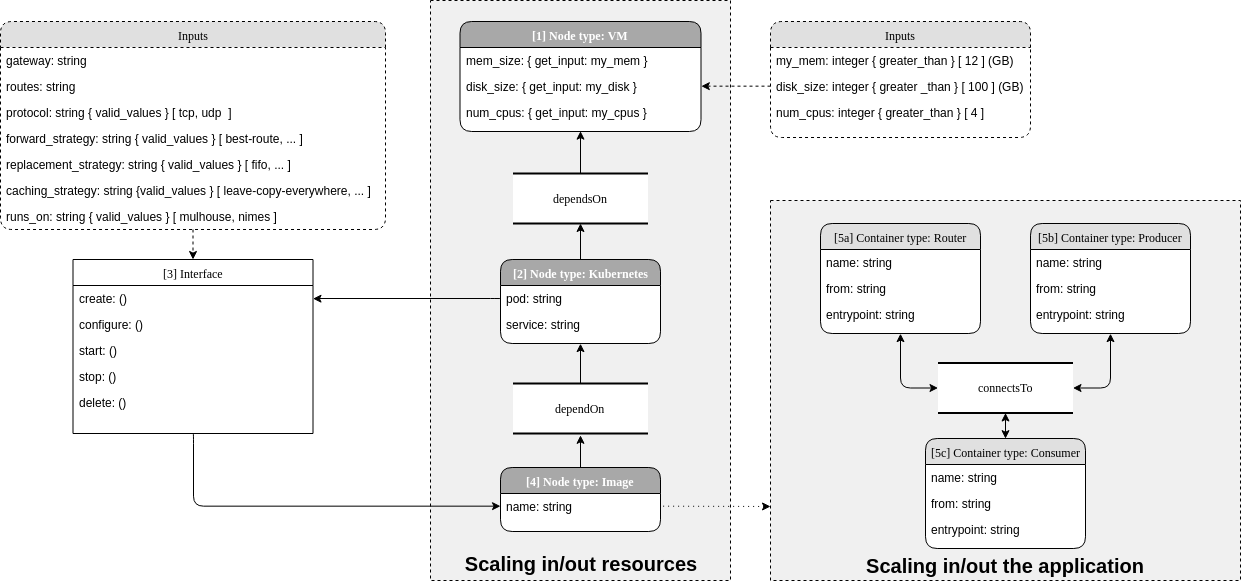
\includegraphics[width=\columnwidth]{Images/tosca-diagram.png}
\caption{TOSCA diagram.}
\label{fig:tosca-diagram}
\end{figure}

In figure \ref{fig:tosca-diagram}, a \gls{tosca} diagram is illustrated. This diagram represents an abstract template description of the \gls{tosca} relationships, in which the grey rectangular boxes are the core scalability factors. As described in section \ref{overview-tosca}, \gls{tosca} consists out of several types; nodes, relationships and interfaces. The scaling properties are highlighted in the rectangular areas. The left area, highlighted as 'scaling in/out resources' contains a dependency chain of several virtual \gls{ndn} functions. This dependency chain is also depicted numerically. Before a pod can be deployed on Kubernetes (step 2 to 5), a VM needs to exist (step 1). This is described by the 'dependsOn' relationship. Furthermore, with the requirements defined in section \ref{planning-requirements}, input constraints are described. These constraints are used by the orchestrator to make sure that the \gls{ndn} infrastructure has sufficient resources available to operate. Once a VM is deployed, the dependency for Kubernetes is satisfied, thus Kubernetes can then be setup (step 2). Kubernetes can then deploy pods by the use of interfaces (step 3). These interfaces feed the containers with environment variables such as the gateway, a list of routes, the transport protocol for \gls{ndn}, the \gls{ndn} strategies and on which Kubernetes node this pod should run. The environment variables are given to the interface via the \gls{tosca} inputs. These environment variables are then used by scripts that run inside the pods to setup \gls{ndn}. Several constraints are set for these environment variables such as which valid transport protocols can be used for \gls{ndn}, which \gls{ndn} strategies are valid and which nodes are available. These constraints are defined with e.g. 'valid\_values' or 'greater\_than' definitions. These constraints help to guide the orchestrator to verify the inputs that are given for the template description. As illustrated in the second gray area 'scaling in/out the application', several pods can be instantiated (step 5a, 5b and 5c) from the image (step 4). These pods enable the virtual \gls{ndn} functions as described in section \ref{planning-architecture}. These pods establish the \gls{ndn} and therefore are connected via the 'connectsTo' relationship. This network expands over to other Kubernetes nodes in the cluster by the use of the Kubernetes built-in overlay network.

\subsection{Proof of concept}
\label{planning-poc}
With the methodology defined, in which scalability and performance requirements are met and a method for deployment is described, a proof of concept was used to test the methodology. The orchestrators mentioned in section \ref{overview-tosca} are still in a prototype phase when combined with a \gls{tosca} parser. Therefore, in our proof of concept we deployed the VMs and Kubernetes nodes manually. In practice the life cycle of also the Kubernetes pods are managed by a \gls{tosca} orchestrator. Without having a \gls{tosca}-ready orchestrator available, steps 2 through 5 in figure \ref{fig:tosca-diagram} were be carried out by Kubernetes exclusively. This was done by defining the configuration properties\footnote{\url{https://github.com/AquaL1te/rp2/blob/master/Kubernetes/expanded-cluster.yml}} of the pods manually. These properties include the \gls{ndn} function name, e.g. router, producer or consumer. And also includes the routes (NDN prefixes) and the associated \gls{ndn} face with the transport protocol to use (TCP or UDP). These parameters were then inserted into the \gls{ndn} \gls{fib} by the scripts that were executed inside the pod\footnote{\url{https://github.com/AquaL1te/rp2/blob/master/Docker/producer/docker-entrypoint.sh}}. The \gls{ndn} strategies were also configured by these scripts. Furthermore, if it is not defined where a pod should be running, Kubernetes will make this decision itself, based on the known resources in the Kubernetes cluster. If for example a Kubernetes node has more memory to spare than other nodes, then Kubernetes will likely decide to spawn the pod there. This Kubernetes node could potentially run in a cloud provider, located in another geographical area. Since the purpose is to provide data distribution through the use of \gls{ndn}, locality becomes a key factor. Therefore, a pod is specifically assigned to a Kubernetes node in order to provide in-network caching in a specific geographical area.

\subsection{Results}
The methods discussed in this section offer a combined way to plan and deploy a data distribution network. McCabe can be used to methodologically adjust the environment to match performance requirements. For the size of this proof of concept the McCabe method is extra overhead. However, the proof of concept is only used to demonstrate the train of thought. The methods discussed can be applied to larger deployments where the McCabe method will be more valuable.

Furthermore, the \gls{ndn} infrastructure life cycle can be managed from Kubernetes. Our proof of concept lacks a \gls{tosca}-ready orchestrator. Therefore, scaling in or out resources to other cloud providers is not demonstrated. However, scaling in or out the \gls{ndn} application is demonstrated. This method allows to reconfigure an \gls{ndn} infrastructure in \gls{nfv}-style by interacting with Kubernetes as the orchestrator. Therefore, the YAML configuration of Kubernetes acts as the \gls{tosca} template description and Kubernetes, which executes this configuration, acts as the orchestrator. In practice the Kubernetes configuration would be generated based on the \gls{tosca} template descriptions and e.g. \gls{drip} would act as the orchestrator. In effect, the \gls{ndn} containers are spawned as \glspl{nfv} which provides scalable management of the \gls{ndn}. These \gls{ndn} \glspl{nfv} may be deployed on a continental or global scale, facilitating a managed distribution network.

In contrast, if \gls{ndn} was deployed without the discussed methods, an alternative would be to have a custom deployments for each cloud environment. Which does not scale in terms of manageability and may create inconsistent deployments and errors. Therefore, that approach also realizes a data distribution network by the use of \gls{ndn}, but does not scale in terms of management and deployment.